\documentclass{article}

\usepackage[brazil]{babel}
\usepackage[utf8]{inputenc}
\usepackage{amsmath}

\usepackage{listings}
\usepackage{mcode}
\usepackage[section]{placeins}

\usepackage{graphicx}

\usepackage{color} %red, green, blue, yellow, cyan, magenta, black, white
\definecolor{mygreen}{RGB}{28,172,0} % color values Red, Green, Blue
\definecolor{mylilas}{RGB}{170,55,241}

\begin{document}

\begin{flushleft}
FUNDAÇÃO GETÚLIO VARGAS \\

Escola de Pós-Graduação em Economia

Teoria Macroeconômica III

Professor: Ricardo de Oliveira Cavalcanti

Monitora: Kátia Aiko Nishiyama Alves

Alunos: Gustavo Bulhões e Samuel Barbosa
\end{flushleft}

\section*{Exercício 02}

Neste exercício temos o modelo clássico de crescimento econômico, cujo problema do planejador
é escolher sequências de consumo $\{c_t\}_{t=0}^{\infty}$ e de capital $\{k_t\}_{t=0}^{\infty}$ que resolvem

\begin{equation}
\begin{aligned}
& \max & & \sum_{t=0}^{\infty} \beta^t u(c_t) \\
& \text{s.a.} & &  c_t + k_{t+1} \leq f(k_t) + (1-\delta) k_t \\
& & &  k_{t+1} \geq 0, c_t \geq 0 \,\, \forall t \geq 0  \\
& & &  k_0 \text{ dado} \\
\end{aligned}
\end{equation}

com $f(k) = k^\alpha$ e $u(c) = \frac{c^{1-\gamma}}{1-\gamma}$.


\subsection*{Item (i)}

Observe que $u(c)$ é monótona crescente em $c$ e, portanto satisfaz a propriedade de não saciedade local.
Logo vale a Lei de Walras, e podemos reescrever a primeira restrição com igualdade,
resolver para $c_t$ e substituir na função objetivo. Desta forma o problema se torna 

\begin{equation}
\begin{aligned}
& \max & & \sum_{t=0}^{\infty} \beta^t u(f(k_t) + (1-\delta) k_t - k_{t+1}) \\
& \text{s.a.} & &  k_{t+1} \geq 0, c_t \geq 0 \,\, \forall t \geq 0  \\
& & &  k_0 \text{ dado} \\
\end{aligned}
\end{equation}

\subsection*{Item (ii)}

Reescrevemos o problema sequencial na forma recursiva, transformando-o na equação funcional

\begin{equation}
\begin{aligned}
V(k) = & \max_{k'} & & u(c) + \beta V(k') \\
& \text{s.a.} & &  c + k' = f(k) + (1-\delta) k \\
& & &  k' \geq 0, c \geq 0 \,\, \\
\end{aligned}
\end{equation}

\subsection*{Item (iii)}

O operador de Bellman associado à equação funcional obtida no item anterior é justamente

\begin{equation}
\begin{aligned}
T(V)(k) = & \max_{k'} & & u(c) + \beta V(k') \\
& \text{s.a.} & &  c + k' = f(k) + (1-\delta) k \\
& & &  k' \geq 0, c \geq 0 \,\, \forall t \geq 0  \\
\end{aligned}
\end{equation}

\subsection*{Item (iv)}

Vamos criar um grid para a variável de estado $k$ no intervalo $[0, 1.25 k_{ss}]$, em que $k_{ss}$ é o nível
de capital de estado estacionário. 

Resolvendo o lado direito da equação funcional $(3)$, já substituindo as funções dadas $u()$ e $f()$, 
obtemos a equação de Euler

$$ c^{-\gamma} = \beta c'^{-\gamma} [\alpha k'^{\alpha-1} + 1 - \delta].$$

No estado estacionário temos que $c' = c$ e $k' = k$. Substituindo na equação anterior obtemos
\begin{equation}
k_{ss} = \left( \frac{1 + \beta (\delta - 1)}{\alpha \beta} \right)^{\frac{1}{\alpha - 1}}.
\end{equation}

Dado $k_{ss}$ podemos construir nosso algoritmo de iteração:

\begin{lstlisting}
% Parametros
alpha = 0.70;
beta = 0.98;
gamma = 2.00;
delta = 0.10;

k_ss = ((1 + beta * (delta - 1))/ alpha * beta )^(1 / (alpha - 1));

% Funcoes
f = @(k) k .^ alpha;
c = @(k, k_linha) max(f(k) + (1 - delta) * k - k_linha, 0);
u = @(c) (c .^ (1 - gamma)) ./ (1 - gamma);

% Grid
n = 1000;
k = linspace(1, 1.25 * k_ss, n);
k_linha = k';
K = repmat(k, n, 1);
K_linha = repmat(k_linha, 1, n);

% Possibilidades de consumo e utilidade
C = c(K, K_linha);
U = u(C);

% Chutes iniciais:
V = zeros(1, n);
g = zeros(1, n);

% Variaveis iteracao
err = 1;
tol = 10^-5;
it = 1;
itmax = 1000;

% Algoritmo de iteracao
while err > tol && it < itmax
    [TV, I] = max(U + beta * repmat(V',1, n));
    err = max(abs((TV - V)));
    V = TV;
    it = it + 1;
end

G = k(I);
\end{lstlisting}

Assim, obtemos as seguintes funções valor e política:

\begin{figure}[!h]
  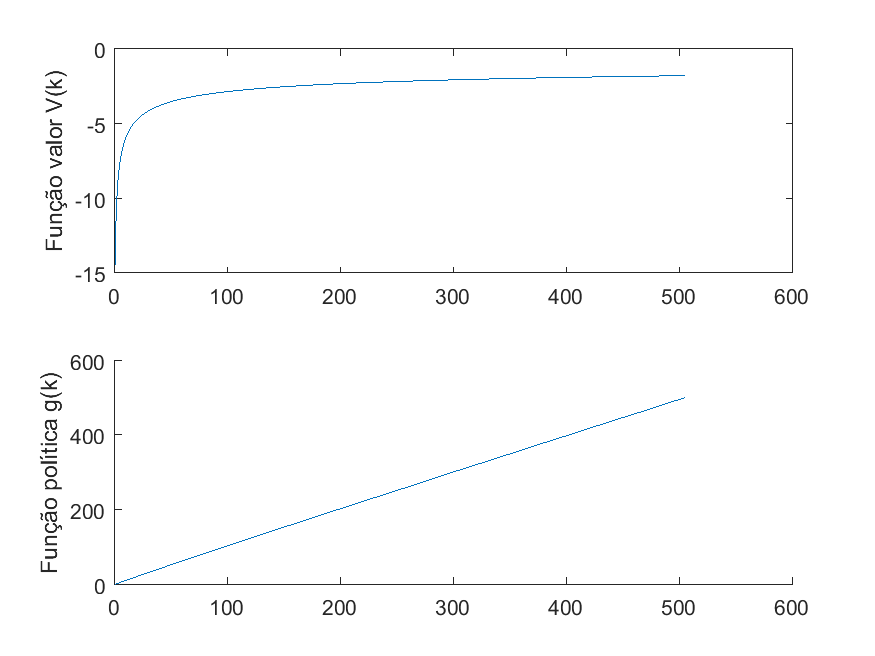
\includegraphics{ex2_1.png}
\end{figure}

\subsection*{Item (v)}

Com $k_0 = 2$, obtemos um nível de capital de estado estacionário $k_{ss} \approx 349.31$, 
ao qual estão associados o nível de produto $y_{ss} \approx 60.29$ e consumo $c_{ss} \approx 25.36$.
O gráfico a seguir mostra a trajetória das escolhas de $k'$ até o $k_{ss}$, quando $k_0 = 2$.

\begin{figure}[!h]
  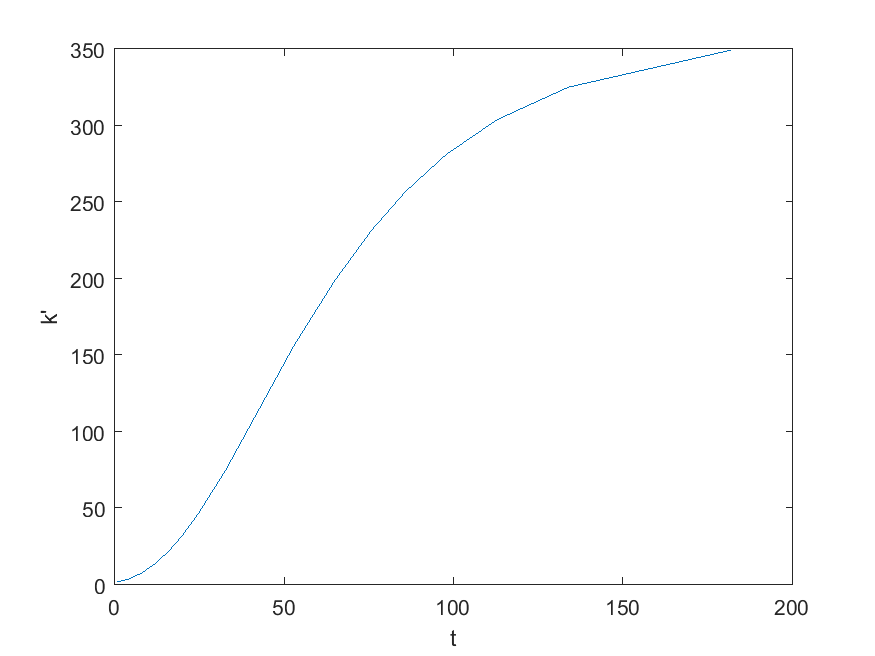
\includegraphics{ex2_2.png}
\end{figure}

\subsection*{Item (vi)}

Na equação (5) temos $k_{ss}$ em função de $\beta$. Avaliando esta equação para valores
de $\beta$ entre $0.7$ e $0.99$ obtemos o gráfico a seguir.

\begin{figure}[!h]
  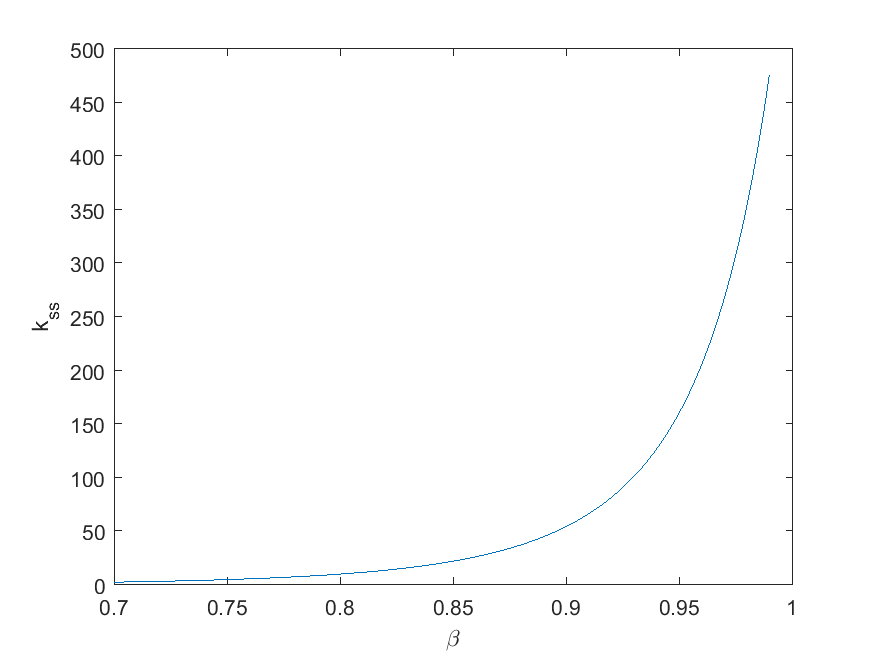
\includegraphics{ex2_3.png}
\end{figure}

\newpage

\subsection*{Item (vii)}

Conforme a equação 5, $k_{ss}$ não depende de $\gamma$.


\end{document}